\chapter{Source Code}

The diagram below represents a structured listing of files and directories involved in the project. It visualises the organisation and hierarchy of the project's components as follows:
\begin{itemize}
    \item \textbf{Rounded Rectangles:} These shapes indicate directories, which are containers that hold files or other directories.
    \item \textbf{Regular Rectangles:} These represent code files within the directories.
    \item \textbf{Connecting Lines:} The lines show the hierarchical relationships between directories and files. If a line connects one rectangle or rounded rectangle to another, it indicates that the item at the arrow's end is contained within the item from which the line originates.
    \item \textbf{Colour Coding:} The colour of each figure signifies its level in the hierarchy. For instance, directories like \textit{backend}, \textit{frontend}, \textit{nginx}, and \textit{AI-models} are all coloured green, indicating they are at the same hierarchical level.
\end{itemize}

The image is high resolution; please enlarge it by pressing \textit{Ctrl} and scrolling up with the mouse to read it clearly.

\begin{figure}
    \centering
    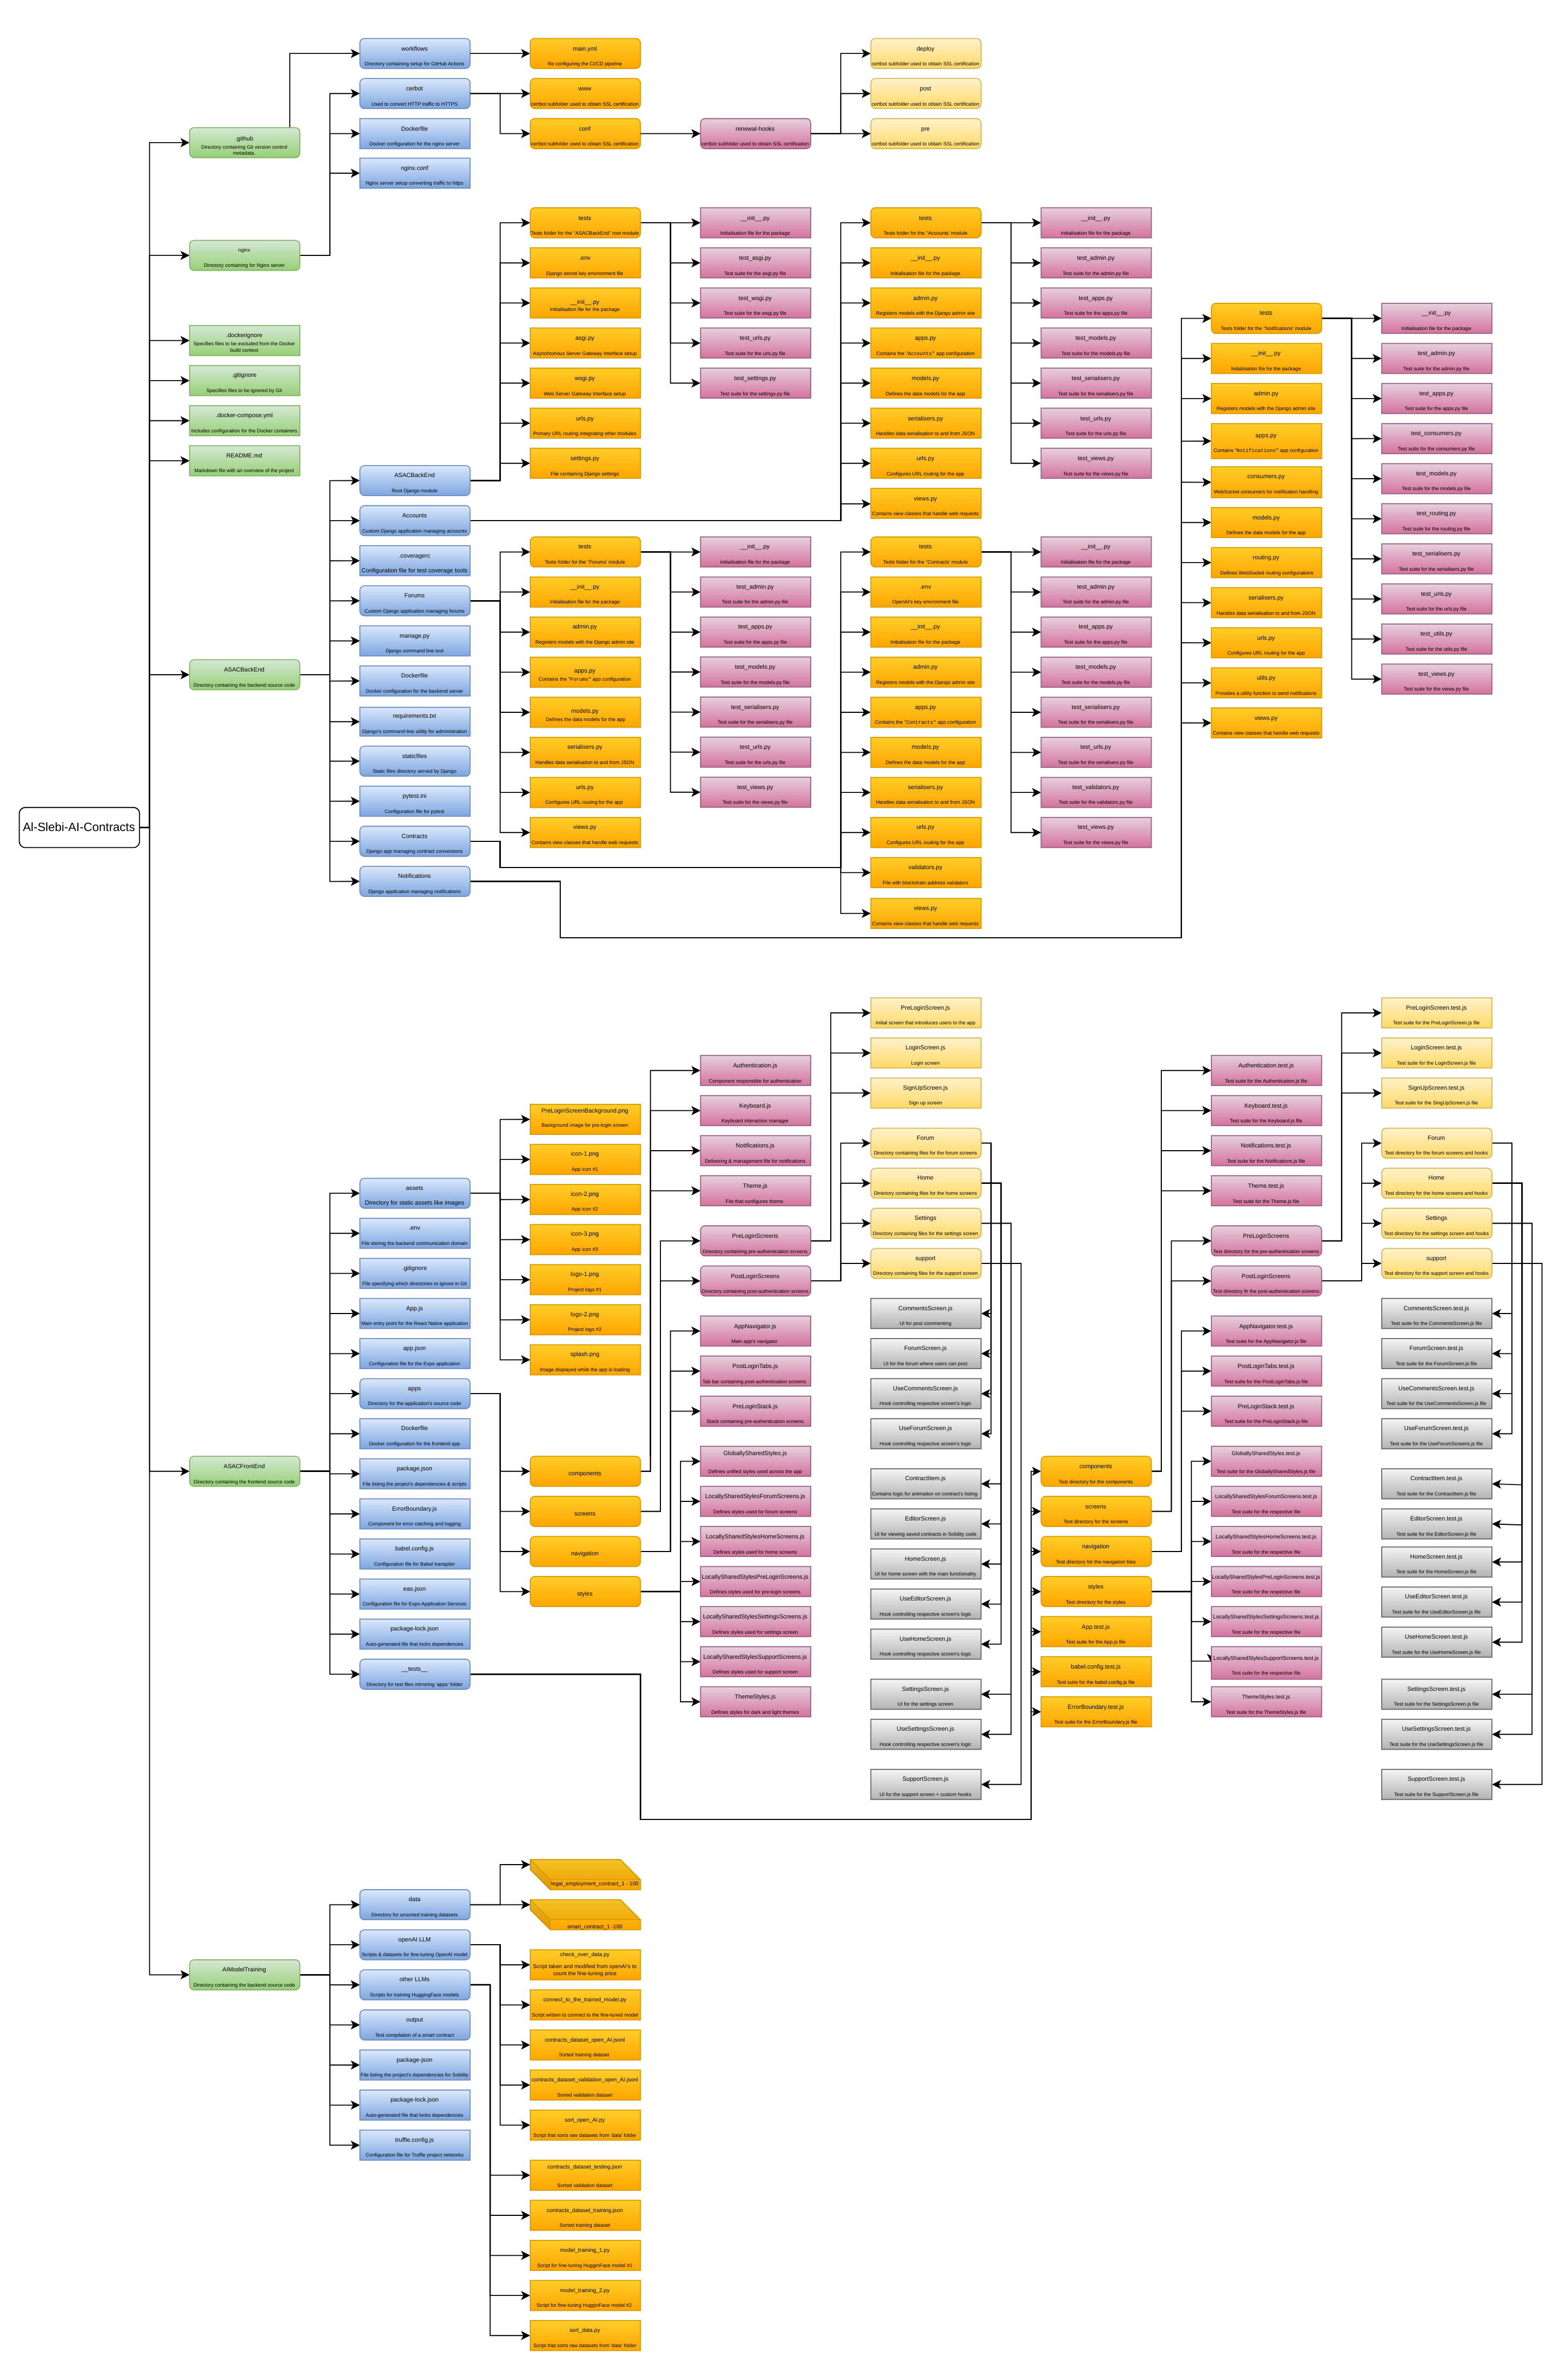
\includegraphics[width=1\linewidth]{LATEX/Appendices/Images/Software/files-listing.png}
    \label{fig:files-listing}
\end{figure}